\chapter[Proposta]{Proposta}

\label{chap:proposta}

Este capítulo visa detalhar a proposta deste Trabalho de Conclusão de Curso, que se baseia na construção de uma ferramenta orientada ao gerenciamento e suporte ao processo da Engenharia de Requisitos. Dentro deste contexto, é apresentada a contextualização da proposta (seção \ref{sec:contextualizacao}), seguido da descrição da ferramenta \textit{iFlow} (seção \ref{sec:sobre_a_ferramenta}), descrevendo a arquitetura de \textit{software} (seção \ref{sec:arquitetura_da_solucao}), utilizada para o desenvolvimento da ferramenta, além das especificidades dos módulos do sistema, seguindo para a apresentação da identidade visual (seção \ref{sec:identidade_visual}) e, por fim, tem-se a apresentação do protótipo de alta fidelidade e do \textit{backlog} da ferramenta (seções \ref{sec:prototipo_de_alta_fidelidade} e \ref{sec:backlog_do_produto}).

\section{Contextualização}

\label{sec:contextualizacao}

A principal justificativa para o desenvolvimento da ferramenta proposta neste trabalho diz respeito a buscar minimizar e evidenciar os problemas associados aos processos da Engenharia de Requisitos.

Reproduzindo um papel essencial no desenvolvimento de produtos de \textit{software}, a Engenharia de Requisitos fornece uma maneira de entender e descrever problemas que precisam de uma solução de \textit{software}. Além disso, é um ramo que está inteiramente ligado ao ciclo de desenvolvimento do \textit{software} \cite{elliott2012software}. Dessa forma, por se tratar de uma área negligenciada por muitos, foi considerada a construção de uma ferramenta que ofereça apoio tecnológico, que viabilize e semi-automatize as etapas da Engenharia de Requisitos, com o propósito de facilitar e melhorar estes processos.

A seguir, tem-se uma descrição mais aprofundada da ferramenta que está sendo elaborada neste Trabalho de Conclusão de Curso.

\section{Sobre a Ferramenta iFlow}

\label{sec:sobre_a_ferramenta}

A ferramenta \textit{iFlow} tem o objetivo de viabilizar e semi-automatizar o processo da Engenharia de Requisitos, de modo a embasar a construção de um produto de \textit{software} e evitar que retrabalhos e desperdícios de tempo ocorram devido ao mau planejamento. Neste sentido, algumas automatizações serão realizadas, de modo a estabelecer e se apoiar no conceito de um \textit{Minimum Viable Product} (MVP). Além disso, a ferramenta confere ênfase às etapas da Engenharia de Requisitos, de forma que, uma vez concluída uma etapa, a próxima será desbloqueada. Dessa forma, a ferramenta será composta por algumas etapas, dentre elas: a) pré-rastreabilidade; b) elicitação; c) modelagem; d) \textit{house of quality}; e) análise; e f) pós-rastreabilidade. 

\subsection{Pré-rastreabilidade}

Nesta primeira etapa, o foco da ferramenta será em aplicar os conceitos propostos em pré-rastreabilidade (seção \ref{sec:pre-rastreabilidade}), e iniciar o processo da Engenharia de Requisitos, descrevendo as primeiras definições do produto de \textit{software} em questão, iniciando o levantamento dos requisitos.

Com esse objetivo, os artefatos usados para esta etapa são o \textit{5W2H} (seção \ref{sec:5w2h}), que sintetiza a ideia inicial do produto, e o \textit{Rich Picture} (seção \ref{sec:rich_picture}), que transcreve visualmente os atores e o fluxo de informações envolvidos no processo.

\subsection{Elicitação}

\label{sec:proc_elicitacao}

Estabelecida a visão geral do produto de \textit{software}, a ferramenta parte para a segunda etapa do processo, que levanta o maior número possível de requisitos. A intenção é que se colete diferentes pontos de vistas em diferentes contextos e com opiniões distintas, visando a aquisição de definições do produto mais ricas e que agregue mais valor para os \textit{stakeholders}.

Dessa forma, na ferramenta, existem diversas propostas de métodos que proporcionam modelos que auxiliam na elicitação dessas funcionalidades. Vale salientar que tais métodos não serão obrigatórios para que o usuário siga para a próxima etapa, mas será evidenciada a importância desta etapa, além de uma confirmação de que as funcionalidades levantadas são suficientes para a construção do produto de \textit{software}.

No contexto de cada ferramental, o usuário tem a possibilidade de adicionar diferentes fontes de dados para compor o artefato, sendo: imagens, vídeos, áudios e documentos de texto. O intuito é que, a partir dessas informações, novas funcionalidades sejam adquiridas.

Por conta da complexidade de cada artefato, são disponibilizadas definições rápidas, cujos objetivos são guiar e conduzir de maneira mais adequada o desenvolvimento. Para estudos mais aprofundados, fontes da literatura reconhecidas são sugeridas na ferramenta.

Neste sentido, os artefatos disponibilizados para viabilizar a etapa da elicitação são:

\begin{itemize}
    \item \textit{Brainstorming} (seção \ref{sec:brainstorming}), que coleta o maior número de ideias acerca do produto de \textit{software};
    \item Questionário (seção \ref{sec:questionario}), que tem o objetivo de coletar o maior número de informações a respeito do tema em questão;
    \item Protótipo de Baixa Fidelidade (\ref{sec:prototipo-def}), que ajuda, de forma visual, na elicitação dos requisitos;
    \item \textit{Storytelling} (seção \ref{sec:storytelling}), que extrai as \textit{features} do sistema em um determinado contexto;
    \item Entrevista (seção \ref{sec:entrevista}), que, de certa forma, traz uma visão mais concreta acerca de um tema pelo fato de se ter uma comunicação mais natural entre os envolvidos, e
    \item Análise de Protocolo (seção \ref{sec:analise-protocolo}), que sintetiza os pensamentos de um usuário e, a partir disso, tem-se a extração de possíveis requisitos do sistema.
\end{itemize}

\subsection{Modelagem}

Com as funcionalidades levantadas, a ferramenta segue para a próxima etapa do processo, que visa colocar em modelos estruturados todas as ideias obtidas na etapa anterior (seção \ref{sec:proc_elicitacao}). Diferentemente da elicitação, que tem uma visão muito aberta e livre para proporcionar um espaço saudável para que a criatividade seja o principal foco, este nível visa chegar em um ponto mais concreto e consistente para a construção de uma aplicação. O propósito, é gerar modelos capazes de representar características ou comportamentos do produto de \textit{software}, que possam guiar todo o processo de desenvolvimento.

Vale destacar a importância deste processo, pois concluída esta etapa, o usuário deve viabilizar uma forma para a construção do produto de \textit{software}. Neste ponto, deve-se ter uma visão mais concreta e definitiva da aplicação que se almeja desenvolver.

Esta etapa é imprescindível, pois aqui são gerados artefatos essenciais para a aplicação que será desenvolvida. Sendo assim, os artefatos usados para esta etapa são o \textit{Backlog} (seção \ref{sec:backlog}), que concentra a lista de defeitos, melhorias solicitadas pelo cliente, funcionalidades, entre outros itens que expressam os requisitos do produto; o NFR \textit{Framework} (seção \ref{sec:nfr}), que sintetiza os requisitos não funcionais do sistema no formato de um grafo, e os Léxicos (\ref{sec:lexicos}), que transcrevem todos os vocábulos utilizados no domínio de uma aplicação.

\subsection{Verificação}

Para evitar retrabalhos e gerar artefatos que estejam os mais corretos e concisos possíveis, esta etapa tem o objetivo de revisar o que foi gerado até o momento (seção \ref{sec:verificacao}). No contexto de cada artefato, existem regras e métodos que devem ser seguidos ou algum objetivo que existe ao realizar aquela atividade. Portanto, para cada um dos artefatos gerados, a ferramenta sugere alguns pontos de checagem para que o usuário revise aquilo que foi elaborado, como propõe \citeauthoronline{design_fagan} (\citeyear{design_fagan}) em seu método de inspeção. Todavia, isso não impede que o usuário defina pontos que ache relevante de avaliar.

Definidos quais pontos são relevantes para a avaliação, o usuário dispõe de uma visualização conjunta do artefato revisado para poder realizar o processo de \textit{inspeção}. Feito isso, a ferramenta apresenta ao usuário métricas de precisão do artefato, viabilizando uma correção dos pontos de melhoria levantados.

\subsection{Pós-rastreabilidade}

Em posse de requisitos modelados e concisos, esta etapa trata de um processo, automático gerado pela ferramenta, que produz um grafo (seção \ref{sec:grafos}) a partir do que foi realizado nas etapas anteriores. Esse artefato, chamado \textit{Backward-from} (seção \ref{sec:pos-rastreabilidade}), mantém um requisito desde sua origem, e mantém a visão obtida no momento que o requisito foi extraído.

\subsection{Priorização}

Esta etapa é de suma importância no contexto do processo da Engenharia de Requisitos, pois nela que será definido o Produto Mínimo Viável (seção \ref{sec:priorizacao}) a partir da \textit{House of Quality} (seção \ref{sec:house_of_quality}), onde se tem a correlação dos requisitos funcionais e não funcionais e seus \textit{softgoals}. Aqui, determina-se quais são as principais funcionalidades do produto de \textit{software}, que devem ser validadas e efetivadas pelo usuário final.

\section{Arquitetura de Software}

\label{sec:arquitetura_da_solucao}

Conforme é observado na Figura \ref{fig:arquitetura}, a arquitetura de \textit{software} proposta inclui a integração de dois módulos: o \textit{front-end} e o \textit{back-end}.

\begin{figure}[H]
    \begin{center}
        \caption{{Arquitetura do \textit{Software} da ferramenta \textit{iFlow}}}
        \label{fig:arquitetura}
        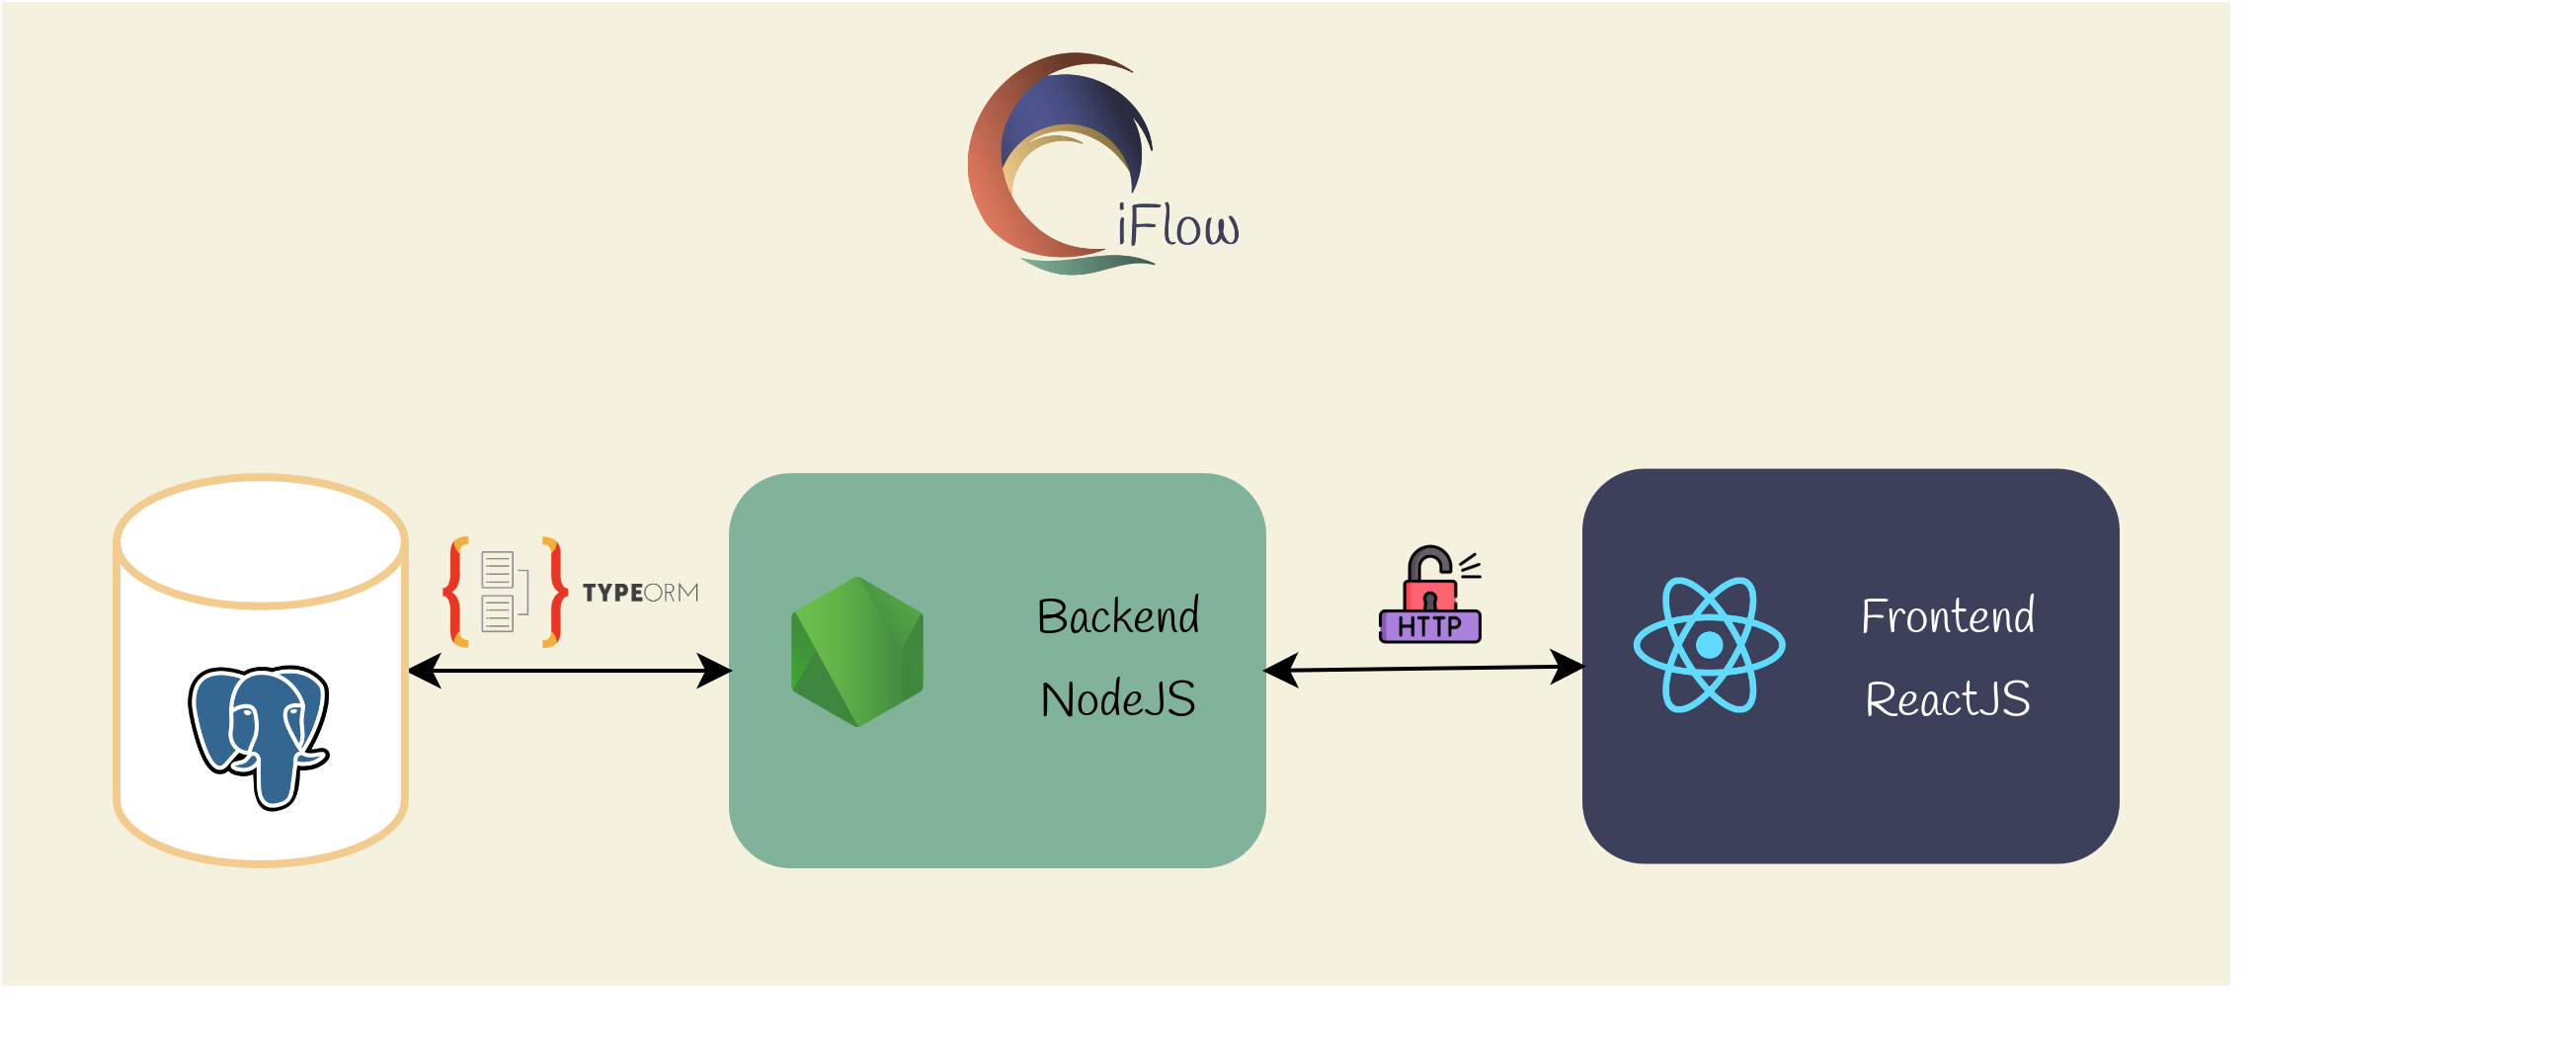
\includegraphics[scale=1.0]{figuras/Proposta/arquitetura.png}
        \legend{Fonte: Autores, 2022.}
    \end{center}
\end{figure}

\subsection{\textit{Front-end}}
O \textit{Front-end} será responsável por realizar as interações com o usuário e com o \textit{back-end}. Além disso, é responsável pela \textit{interface} da ferramenta utilizando recursos \textit{HTML} e \textit{CSS} com o \textit{framework} \textit{React}. Sendo assim, essas tecnologias foram escolhidas devido ao grande suporte que elas oferecem para a construção de \textit{interfaces} de usuário interativas, descritas com mais detalhes no Capítulo \ref{chap:referencial_tecnologico}.

\subsection{\textit{Back-end}}
O \textit{Back-end} será responsável por realizar a conexão com o banco de dados; armazena os dados que serão consumidos ou manipulados pelo \textit{software}, e por realizar o tratamento dos dados. Dessa forma, foi escolhida a tecnologia \textit{Node.js} visando realizar a comunicação entre as camadas de banco de dados e de \textit{front-end}. A tecnologia é descrita com mais detalhes no Capítulo \ref{chap:referencial_tecnologico}.

\section{Identidade Visual}

\label{sec:identidade_visual}

A Identidade Visual é um conjunto de elementos gráficos e visuais, com o intuito de mostrar os principais elementos do seu produto e seus valores. Com o intuito de dar uma identidade visual para a ferramenta \textit{iFlow}, foi elaborado um manual que elenca os logotipos, as cores, a tipografia e os símbolos definidos para o projeto. Esse manual está descrito com maiores detalhes no Apêndice \ref{apendice:identidade_visual}.

\subsection{Logotipo}
O logotipo da ferramenta é a representação de ondas buscando transmitir a noção do processo proveniente da Engenharia de Requisitos, conforme pode-se observar na Figura \ref{fig:logotipo}.

\begin{figure}[H]
    \begin{center}
        \caption{{Logotipo da Ferramenta \textit{iFlow}}}
        \label{fig:logotipo}
        
\includegraphics[scale=1.0]{figuras/Proposta/logotipo.png}
        \legend{Fonte: Autores, 2022.}
    \end{center}
\end{figure}

\section{Diagramas da Aplicação}

\label{sec:diagramas_da_aplicacao}

\subsection{Diagramas de Banco de Dados}

Os diagramas de Banco de Dados visam modelar como os dados serão armazenados pela aplicação. O DE-R (Figura \ref{fig:diagrama_conceitual}) é a representação gráfica e a principal ferramenta de visualização dos relacionamentos entre as entidades do sistema. Já o DL (Figura \ref{fig:diagrama_logico}) descreve como os dados serão armazenados no banco, além dos seus relacionamentos.

\begin{figure}[H]
    \begin{center}
        \caption{{DE-R do Banco de Dados do \textit{iFlow}}}
        \label{fig:diagrama_conceitual}
        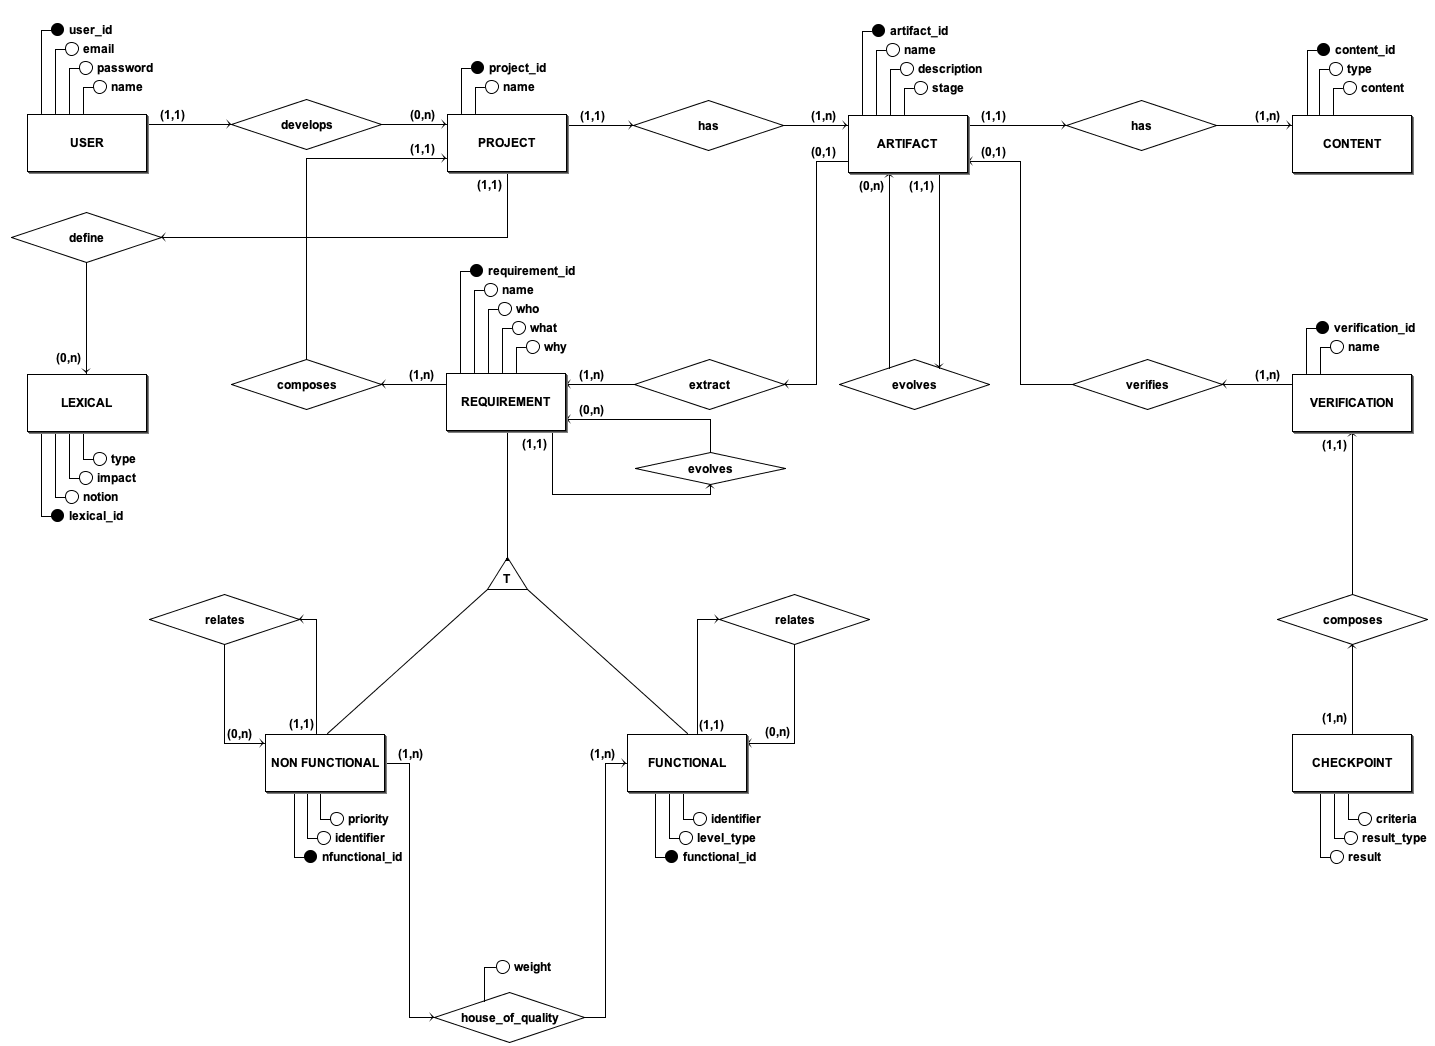
\includegraphics[scale=0.31]{figuras/Proposta/Conceitual_iFlow.png}
        \legend{Fonte: Autores, 2022.}
    \end{center}
\end{figure}

\begin{figure}[H]
    \begin{center}
        \caption{{DL do Banco de Dados do \textit{iFlow}}}
        \label{fig:diagrama_logico}
        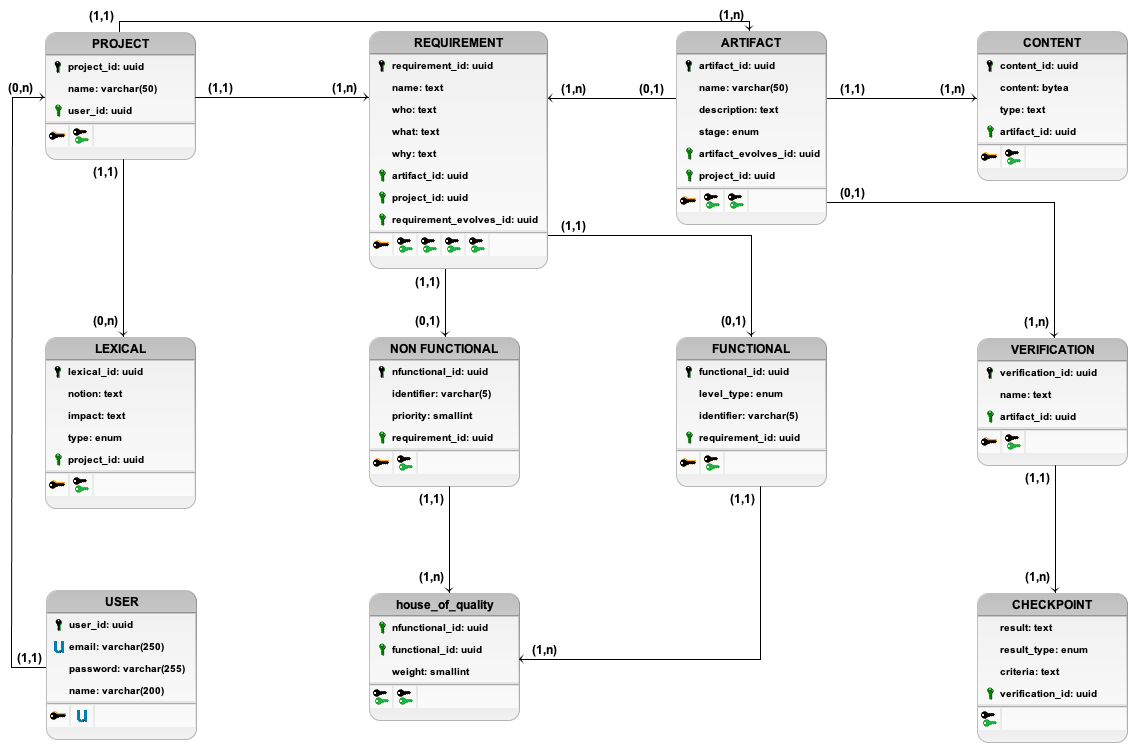
\includegraphics[scale=0.37]{figuras/Proposta/Lógico_iFlow.png}
        \legend{Fonte: Autores, 2022.}
    \end{center}
\end{figure}

O código que cria a base de dados da Ferramenta \textit{iFlow} está disponível no Apêndice \ref{ap:db_sql}.

\subsection{Diagrama de Pacotes}

O Diagrama de Pacotes é representado como um esquema estático, possibilitando a visualização e a organização do projeto de maneira mais adequada e simplificada, proporcionando uma visão em módulos, facilitando o entendimento do projeto durante o desenvolvimento e em possíveis manutenções. Dessa forma, os diagramas das Figuras \ref{fig:pacotes_backend} e \ref{fig:pacotes_frontend} procuram detalhar a organização interna dos pacotes, quanto aos diferentes módulos da ferramenta, \textit{Front-end} e \textit{Back-end}.

\begin{figure}[H]
    \begin{center}
        \caption{{Diagrama de Pacotes do \textit{Backend} do \textit{iFlow}}}
        \label{fig:pacotes_backend}
        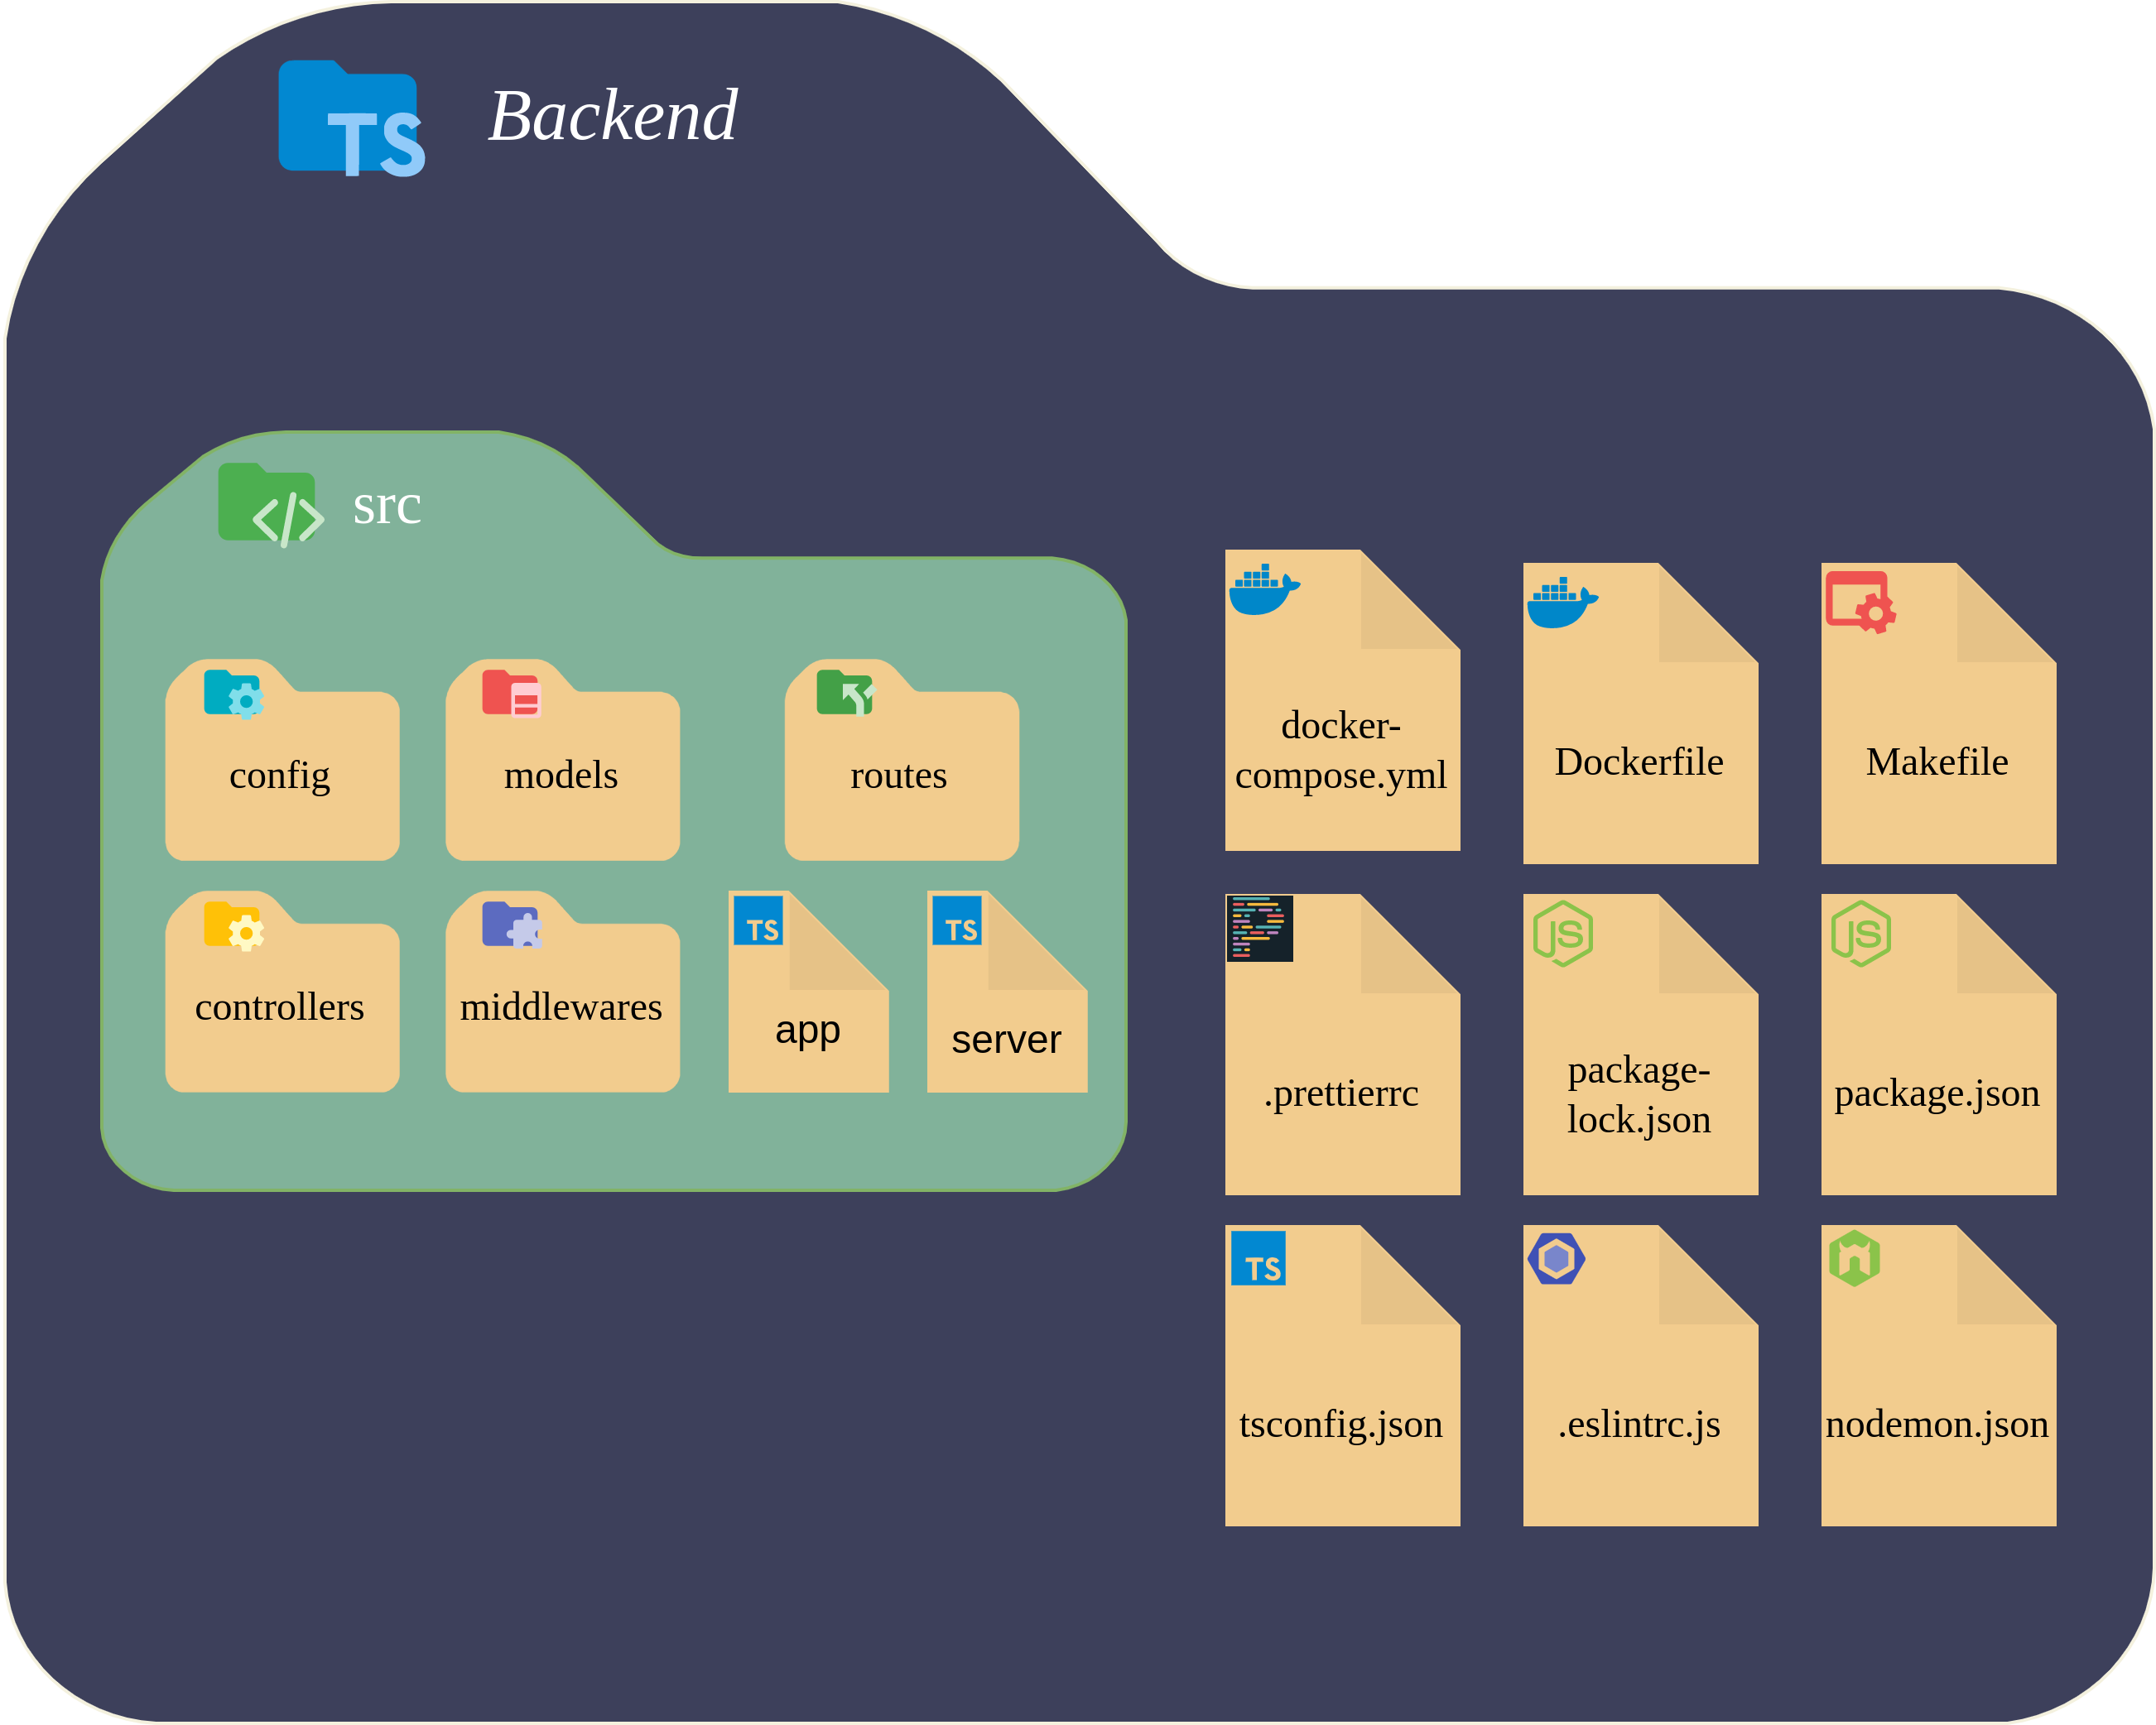
\includegraphics[scale=0.7]{figuras/Proposta/Diagrama_de_Pacotes-Backend.png}
        \legend{Fonte: Autores, 2022.}
    \end{center}
\end{figure}

\begin{figure}[H]
    \begin{center}
        \caption{{Diagrama de Pacotes do \textit{Frontend} do \textit{iFlow}}}
        \label{fig:pacotes_frontend}
        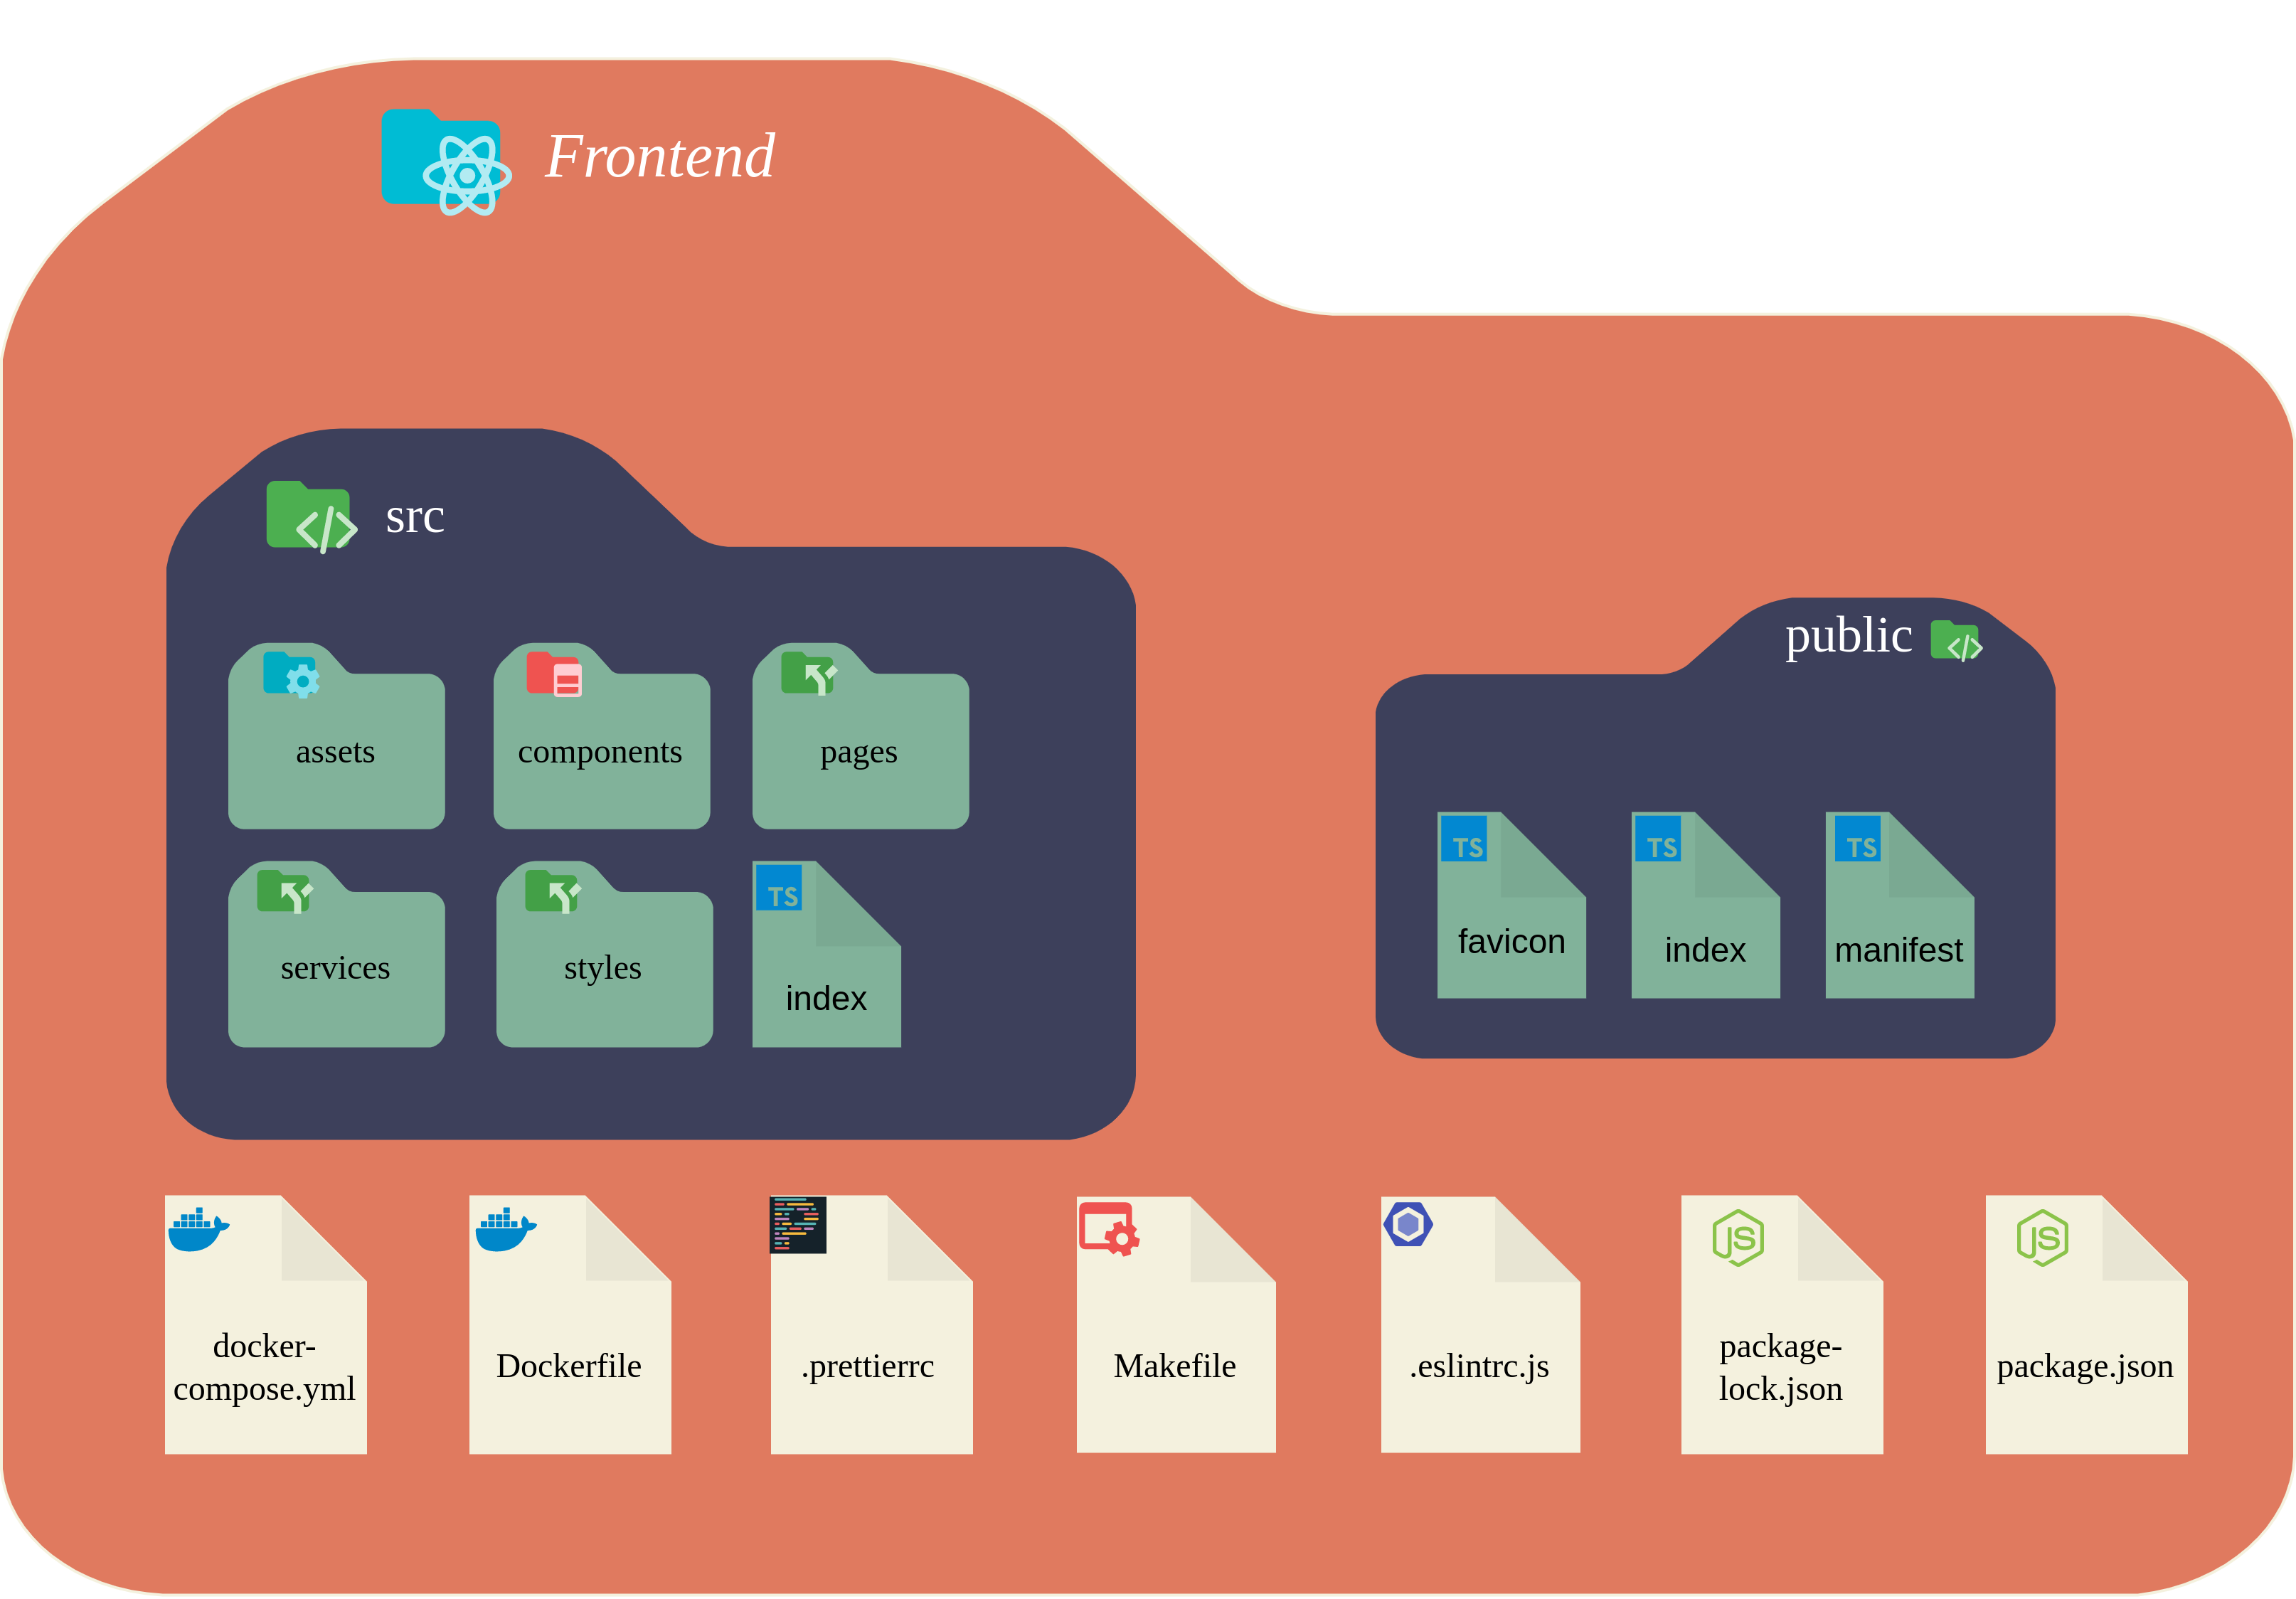
\includegraphics[scale=0.58]{figuras/Proposta/Diagrama_de_Pacotes-Frontend.png}
        \legend{Fonte: Autores, 2022.}
    \end{center}
\end{figure}

\section{Protótipo de Alta Fidelidade}

\label{sec:prototipo_de_alta_fidelidade}

Um protótipo de alta fidelidade deve se aproximar ao máximo dos aspectos visuais e funcionais do produto final, incluindo o conteúdo, fluxo de navegação e interações. São muito utilizados para testes e validação com usuários, ou para apresentar uma ideia. Objetivamente, a ideia do protótipo é saber como a ferramenta funcionará \cite{hf_prototype}.

Com este intuito, foi elaborado um Protótipo de Alta Fidelidade navegável, na plataforma \href{https://www.figma.com/}{Figma}. Contudo, a quantidade de telas geradas foi demasiadamente grande e não haveria a possibilidade de realizar a navegação entre telas. Por isso, foi decidido não adicionar as imagens neste documento, optando-se por disponibilizar o enlace para ser acessado \textit{on-line}: \href{https://www.figma.com/proto/8itTrODQ9x6DeKR1nVluW4/TCC---iFlow?node-id=62\:38&scaling=scale-down&page-id=0\:1&starting-point-node-id=62\:38}{Protótipo de Alta Fidelidade do iFlow}.

\section{\textit{Backlog} do Produto}

\label{sec:backlog_do_produto}

Com o intuito de guiar o processo de desenvolvimento da ferramenta para o TCC2, foi desenvolvido um \textit{backlog} com os requisitos necessários para compor a aplicação. As definições e a tabela foram colocadas no Apêndice \ref{ap:backlog}.

\section{Resumo do Capítulo}

Neste capítulo, foi apresentada a proposta deste Trabalho de Conclusão de Curso, que consiste no desenvolvimento de uma ferramenta que possibilite a semiautomatização, conferindo apoio nos processos da Engenharia de Requisitos. Para isso, foi apresentada a contextualização da proposta; uma seção abordando a ferramenta \textit{iFlow} e seus principais pontos; a arquitetura da solução, com detalhamento dos componentes presentes na mesma; a identidade visual da ferramenta e os diagramas da ferramenta proposta, sendo o Diagrama de Banco de Dados e o Diagrama de Pacotes. Vale ressaltar que, ao longo do desenvolvimento do projeto, ajustes na solução prevista podem ser necessários. Nesse caso, os mesmos serão devidamente apresentados e justificados.